%%%%%%%%%%%%%%%%%%%%%%%%%%%%%%%%%%%%%%%%%
% Short Sectioned Assignment LaTeX Template Version 1.0 (5/5/12)
% This template has been downloaded from: http://www.LaTeXTemplates.com
% Original author:  Frits Wenneker (http://www.howtotex.com)
% License: CC BY-NC-SA 3.0 (http://creativecommons.org/licenses/by-nc-sa/3.0/)
%%%%%%%%%%%%%%%%%%%%%%%%%%%%%%%%%%%%%%%%%

%----------------------------------------------------------------------------------------
%	PACKAGES AND OTHER DOCUMENT CONFIGURATIONS
%----------------------------------------------------------------------------------------

\documentclass[paper=a4, fontsize=11pt]{scrartcl} % A4 paper and 11pt font size

% ---- Entrada y salida de texto -----

\usepackage[T1]{fontenc} % Use 8-bit encoding that has 256 glyphs
\usepackage[utf8]{inputenc}

% ---- Idioma --------

\usepackage[spanish, es-tabla]{babel} % Selecciona el español para palabras introducidas automáticamente, p.ej. "septiembre" en la fecha y especifica que se use la palabra Tabla en vez de Cuadro

% ---- Otros paquetes ----

\usepackage{amsmath,amsfonts,amsthm} % Math packages
\usepackage{graphics,graphicx, floatrow} %para incluir imágenes y notas en las imágenes
\usepackage{graphics,graphicx, float} %para incluir imágenes y colocarlas
\usepackage{hyperref} % url in references

% Para hacer tablas comlejas
\usepackage{multirow}
\usepackage{threeparttable}

\usepackage{fancyhdr} % Custom headers and footers
\pagestyle{fancyplain} % Makes all pages in the document conform to the custom headers and footers
\fancyhead{} % No page header - if you want one, create it in the same way as the footers below
\fancyfoot[L]{} % Empty left footer
\fancyfoot[C]{} % Empty center footer
\fancyfoot[R]{\thepage} % Page numbering for right footer
\renewcommand{\headrulewidth}{0pt} % Remove header underlines
\renewcommand{\footrulewidth}{0pt} % Remove footer underlines
\setlength{\headheight}{13.6pt} % Customize the height of the header

\numberwithin{equation}{section} % Number equations within sections (i.e. 1.1, 1.2, 2.1, 2.2 instead of 1, 2, 3, 4)
\numberwithin{figure}{section} % Number figures within sections (i.e. 1.1, 1.2, 2.1, 2.2 instead of 1, 2, 3, 4)
\numberwithin{table}{section} % Number tables within sections (i.e. 1.1, 1.2, 2.1, 2.2 instead of 1, 2, 3, 4)

\setlength\parindent{0pt} % Removes all indentation from paragraphs - comment this line for an assignment with lots of text

\newcommand{\horrule}[1]{\rule{\linewidth}{#1}} % Create horizontal rule command with 1 argument of height

\usepackage{textcomp}

%----------------------------------------------------------------------------------------
%	DATOS
%----------------------------------------------------------------------------------------

\newcommand{\myName}{Francisco Javier Bolívar Lupiáñez}
\newcommand{\myDegree}{Máster en Ingeniería Informática}
\newcommand{\myFaculty}{E. T. S. de Ingenierías Informática y de Telecomunicación}
\newcommand{\myDepartment}{Ciencias de la Computación e Inteligencia Artificial}
\newcommand{\myUniversity}{\protect{Universidad de Granada}}
\newcommand{\myLocation}{Granada}
\newcommand{\myTime}{\today}
\newcommand{\myTitle}{Práctica 1}
\newcommand{\mySubtitle}{Redes neuronales: Reconocimiento óptico de caracteres MNIST}
\newcommand{\mySubject}{Inteligencia Computacional}
\newcommand{\myYear}{2016-2017}

%----------------------------------------------------------------------------------------
%	PORTADA
%----------------------------------------------------------------------------------------


\title{	
	\normalfont \normalsize 
	\textsc{\textbf{\mySubject \space (\myYear)} \\ \myDepartment} \\[20pt] % Your university, school and/or department name(s)
	\textsc{\myDegree \\[10pt] \myFaculty \\ \myUniversity} \\[25pt]
	\horrule{0.5pt} \\[0.4cm] % Thin top horizontal rule
	\huge \myTitle: \mySubtitle \\ % The assignment title
	\horrule{2pt} \\[0.5cm] % Thick bottom horizontal rule
	\normalfont \normalsize
}

\author{\myName} % Nombre y apellidos

\date{\myTime} % Incluye la fecha actual
%----------------------------------------------------------------------------------------
%	INDICE
%----------------------------------------------------------------------------------------

\begin{document}
	
\setcounter{page}{0}

\maketitle % Muestra el Título
\thispagestyle{empty}

\newpage %inserta un salto de página

\tableofcontents % para generar el índice de contenidos

%\listoffigures

\newpage

%----------------------------------------------------------------------------------------
%	DOCUMENTO
%----------------------------------------------------------------------------------------

\section{Introducción}

Las redes neuronales son muy utilizadas para el reconocimiento de patrones. Y se podría decir que el hola mundo de éstas es la base de datos MNIST \footnote{\url{http://yann.lecun.com/exdb/mnist/}} para el Reconocimiento Óptico de Caracteres (OCR).
\\ \\
Esta base de datos contiene 60.000 imágenes de números (Figura \ref{fig:sample-mnist-data}) para entrenar la red neuronal y 10.000 para probarla. Cada una de estas imágenes de un tamaño de 28x28 píxeles.
\begin{figure}[H]
	\centering
	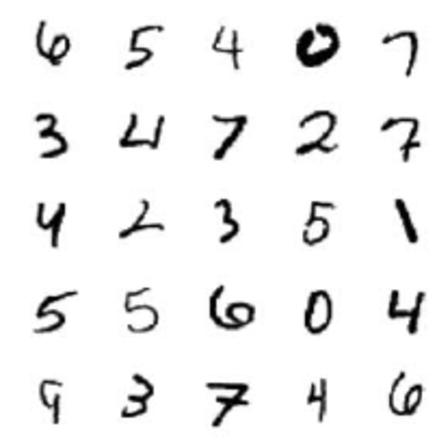
\includegraphics[width=6cm]{img/sample-mnist-data}
	\caption{Muestra de algunas de las imágenes de números de la base de datos MNIST}
	\label{fig:sample-mnist-data}
\end{figure}
El objetivo de esta práctica es el estudio del uso de distintas redes neuronales para resolver este problema obteniendo el mínimo porcentaje de error posible.
\\ \\
Para ello, se ha realizado durante varias semanas de clase una introducción desde cero de los distintos métodos que podrían utilizarse. Desde un perceptrón simple hasta redes neuronales convolucionales.

\section{Implementación}

La primera decisión que tuve que tomar fue la de qué lenguaje de programación y librerías utilizar. 
\\ \\
Me hacía ilusión \textbf{realizar una red neuronal sin la ayuda de ninguna librería}, por lo que descarté desde un principio la posibilidad de utilizar alguna librería que me pudiese facilitar el trabajo. 
\\ \\
Dado que se proporcionaron algoritmos para la lectura de los datos de MNIST tanto en Java y MatLab, y no conocía ni había usado antes MatLab, \textbf{decidí usar Java}, un lenguaje de programación que domino con soltura después de varios años de experiencia utilizando para distintas prácticas del grado en ingeniería informática.

\subsection{Una primera solución}

La primera solución que probé para resolver el problema, fue la idea que se presentó el primer día de clase, que trataba de \textbf{crear plantillas según las imágenes de entrenamiento}.
\\ \\
Para entrenar, se recorre cada imagen de entrenamiento y, para cada píxel de la imagen, se ve si tiene tinta o no. Si la tiene, se le suma valor a ese píxel en la plantilla con el mismo índice que la etiqueta de la imagen que se está utilizando para entrenar. Si por el contrario no tiene tinta, lo que se hace es restar.
\\ \\
Una vez entrenada, para ver cuál es el número de una imagen de test, por cada píxel con tinta, se ve si se tiene un valor positivo en cada una de las plantillas, y para el que tenga, se le añade un voto. Una vez recorridos todos los píxeles de la imagen, se hace un recuento de votos, y la plantilla que haya obtenido más votos es la que indica el número que se ve en la imagen.
\\ \\
Esta solución. Al iniciar siempre a cero los valores de las plantillas generaba siempre el mismo \textbf{resultado que era el de un 55,8\%}.
\\ \\
Esta tasa de error \textbf{se redujo hasta un 34,09\% al reforzar los píxeles con tinta} sumando 5 en vez de 1 a la plantilla.

\subsection{\textit{Backpropagation}}

La falta de tiempo por la proximidad de la fecha de entrega tras haber dejado aparcada la práctica varias semanas hizo que pasase directamente de esta primera y muy básica solución a la realización de algo que pudiese bajar del 10\% de error. Por lo que pasé de realizar el perceptrón simple con el que obtendría unos resultados similares a los ya obtenidos y me puse manos a la obra con una red neuronal multicapa con \textit{backpropagation}.

\subsubsection{\textit{Backpropagation} simple con una sola época}

Realicé una primera implementación con la siguiente topología:
\begin{itemize}
	\item \textbf{Número de capas}: Tres capas. Capa de entrada, oculta y de salida
	\item \textbf{Tamaño de capa de entrada}: 28x28. Tantas neuronas como píxeles en la imagen
	\item \textbf{Tamaño de capa de salida}: 10. Tantas neuronas como posibles soluciones. Si tiene valor 1, o lo ronda, significará que el número de la imagen corresponde al índice de esa neurona
	\item \textbf{Pesos}: Un peso por cada conexión entre neurona inicializados entre -1,67 y 1,67
	\item \textbf{Función de activación}: Sigmoidal
	\item \textbf{Ratio de aprendizaje}: 0,7
	\item \textbf{Tipo de aprendizaje}: Estocástico. Reajuste de pesos tras cada imagen
\end{itemize}
Los resultados obtenidos tras una sola época eran malos, rondaban el 90\%. Y no solo era por inicializar los pesos de las neuronas a unos valores tan grandes, ni por ese ratio excesivamente grande. El problema era que había calculado mal las funciones utilizadas para reajustar los pesos.
\\ \\
Para solucionar esto estuve leyendo varios artículos \cite{backpropagation-de} \cite{backpropagation-au} que me ayudaron a encontrar los fallos que tenía. Antes de empezar a depurar los fallos, cambié el número de neuronas en la capa oculta para que el tiempo de entrenamiento fuese más corto y usé 100 neuronas en ésta capa.
\\ \\
Una vez resueltos estos fallos, añadido el sesgo y su peso (\textit{bias}) a cada neurona y cambiado los valores tanto de inicialización de los pesos (-0,1 y 0,1) y el ratio de aprendizaje (0,17), en una sola época se obtuvo un \textbf{resultado que rondó el 10\%}.

\subsubsection{\textit{Backpropagation} usando momentos y varias épocas}

Para mejorar los resultados podía aplicar \textit{softmax}, pero el tiempo con el que contaba era escaso, por lo que el siguiente paso que podía dar sin agotar mucho tiempo era el del uso de momentos.
\\ \\
No obstante, el uso que hice de este método no es el que se hace de él normalmente. Pues en lugar de variar el valor del momento de 0,5 al principio hasta 0,9 lo iniciaba directamente a 0,9. No se aprovecha de esta forma todas las ventajas que se podrían llegar a tener durante la oscilación en el gradiente descendente, pero sí mejoraba los resultados \textbf{de en torno a un 4\% tras diez épocas con la topología anterior} (con 256 neuronas en la capa oculta) \textbf{a un 2\%} solo añadiendo la constante del momento, multiplicada por la variación del peso anterior, a la variación del peso actual \cite{backpropagation-au}.

\subsubsection{Topología de la red neuronal final}

La red neuronal final se podría definir como una red neuronal multicapa, que usa una función de activación sigmoidal, \textit{backpropagation} con momentos y aprendizaje estocástico.

\subsubsection{Ajustando constantes}

Lala

\section{Resultados}

Lala

\section{Conclusiones}

Lala


%----------------------------------------------------------------------------------------
%	REFERENCIAS
%----------------------------------------------------------------------------------------

\newpage

\bibliography{referencias} %archivo referencias.bib que contiene las entradas 
\bibliographystyle{plain} % hay varias formas de citar

\end{document}